\documentclass[1p]{elsarticle_modified}
%\bibliographystyle{elsarticle-num}

%\usepackage[colorlinks]{hyperref}
%\usepackage{abbrmath_seonhwa} %\Abb, \Ascr, \Acal ,\Abf, \Afrak
\usepackage{amsfonts}
\usepackage{amssymb}
\usepackage{amsmath}
\usepackage{amsthm}
\usepackage{scalefnt}
\usepackage{amsbsy}
\usepackage{kotex}
\usepackage{caption}
\usepackage{subfig}
\usepackage{color}
\usepackage{graphicx}
\usepackage{xcolor} %% white, black, red, green, blue, cyan, magenta, yellow
\usepackage{float}
\usepackage{setspace}
\usepackage{hyperref}

\usepackage{tikz}
\usetikzlibrary{arrows}

\usepackage{multirow}
\usepackage{array} % fixed length table
\usepackage{hhline}

%%%%%%%%%%%%%%%%%%%%%
\makeatletter
\renewcommand*\env@matrix[1][\arraystretch]{%
	\edef\arraystretch{#1}%
	\hskip -\arraycolsep
	\let\@ifnextchar\new@ifnextchar
	\array{*\c@MaxMatrixCols c}}
\makeatother %https://tex.stackexchange.com/questions/14071/how-can-i-increase-the-line-spacing-in-a-matrix
%%%%%%%%%%%%%%%

\usepackage[normalem]{ulem}

\newcommand{\msout}[1]{\ifmmode\text{\sout{\ensuremath{#1}}}\else\sout{#1}\fi}
%SOURCE: \msout is \stkout macro in https://tex.stackexchange.com/questions/20609/strikeout-in-math-mode

\newcommand{\cancel}[1]{
	\ifmmode
	{\color{red}\msout{#1}}
	\else
	{\color{red}\sout{#1}}
	\fi
}

\newcommand{\add}[1]{
	{\color{blue}\uwave{#1}}
}

\newcommand{\replace}[2]{
	\ifmmode
	{\color{red}\msout{#1}}{\color{blue}\uwave{#2}}
	\else
	{\color{red}\sout{#1}}{\color{blue}\uwave{#2}}
	\fi
}

\newcommand{\Sol}{\mathcal{S}} %segment
\newcommand{\D}{D} %diagram
\newcommand{\A}{\mathcal{A}} %arc


%%%%%%%%%%%%%%%%%%%%%%%%%%%%%5 test

\def\sl{\operatorname{\textup{SL}}(2,\Cbb)}
\def\psl{\operatorname{\textup{PSL}}(2,\Cbb)}
\def\quan{\mkern 1mu \triangleright \mkern 1mu}

\theoremstyle{definition}
\newtheorem{thm}{Theorem}[section]
\newtheorem{prop}[thm]{Proposition}
\newtheorem{lem}[thm]{Lemma}
\newtheorem{ques}[thm]{Question}
\newtheorem{cor}[thm]{Corollary}
\newtheorem{defn}[thm]{Definition}
\newtheorem{exam}[thm]{Example}
\newtheorem{rmk}[thm]{Remark}
\newtheorem{alg}[thm]{Algorithm}

\newcommand{\I}{\sqrt{-1}}
\begin{document}

%\begin{frontmatter}
%
%\title{Boundary parabolic representations of knots up to 8 crossings}
%
%%% Group authors per affiliation:
%\author{Yunhi Cho} 
%\address{Department of Mathematics, University of Seoul, Seoul, Korea}
%\ead{yhcho@uos.ac.kr}
%
%
%\author{Seonhwa Kim} %\fnref{s_kim}}
%\address{Center for Geometry and Physics, Institute for Basic Science, Pohang, 37673, Korea}
%\ead{ryeona17@ibs.re.kr}
%
%\author{Hyuk Kim}
%\address{Department of Mathematical Sciences, Seoul National University, Seoul 08826, Korea}
%\ead{hyukkim@snu.ac.kr}
%
%\author{Seokbeom Yoon}
%\address{Department of Mathematical Sciences, Seoul National University, Seoul, 08826,  Korea}
%\ead{sbyoon15@snu.ac.kr}
%
%\begin{abstract}
%We find all boundary parabolic representation of knots up to 8 crossings.
%
%\end{abstract}
%\begin{keyword}
%    \MSC[2010] 57M25 
%\end{keyword}
%
%\end{frontmatter}

%\linenumbers
%\tableofcontents
%
\newcommand\colored[1]{\textcolor{white}{\rule[-0.35ex]{0.8em}{1.4ex}}\kern-0.8em\color{red} #1}%
%\newcommand\colored[1]{\textcolor{white}{ #1}\kern-2.17ex	\textcolor{white}{ #1}\kern-1.81ex	\textcolor{white}{ #1}\kern-2.15ex\color{red}#1	}

{\Large $\underline{12n_{0823}~(K12n_{0823})}$}

\setlength{\tabcolsep}{10pt}
\renewcommand{\arraystretch}{1.6}
\vspace{1cm}\begin{tabular}{m{100pt}>{\centering\arraybackslash}m{274pt}}
\multirow{5}{120pt}{
	\centering
	\includegraphics[width=112pt]{../../../GIT/diagram.site/Diagrams/png/2912_12n_0823.png}\\
\ \ \ A knot diagram\footnotemark}&
\allowdisplaybreaks
\textbf{Linearized knot diagam} \\
\cline{2-2}
 &
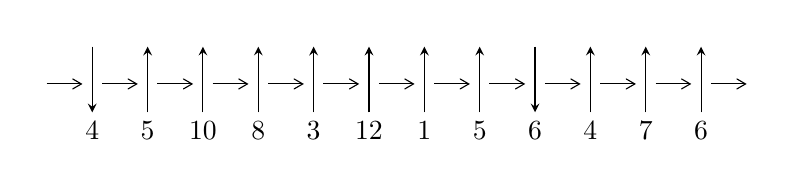
\begin{tikzpicture}[x=20pt, y=17pt]
	% nodes
	\node (C0) at (0, 0) {};
	\node (C1) at (1, 0) {};
	\node (C1U) at (1, +1) {};
	\node (C1D) at (1, -1) {4};

	\node (C2) at (2, 0) {};
	\node (C2U) at (2, +1) {};
	\node (C2D) at (2, -1) {5};

	\node (C3) at (3, 0) {};
	\node (C3U) at (3, +1) {};
	\node (C3D) at (3, -1) {10};

	\node (C4) at (4, 0) {};
	\node (C4U) at (4, +1) {};
	\node (C4D) at (4, -1) {8};

	\node (C5) at (5, 0) {};
	\node (C5U) at (5, +1) {};
	\node (C5D) at (5, -1) {3};

	\node (C6) at (6, 0) {};
	\node (C6U) at (6, +1) {};
	\node (C6D) at (6, -1) {12};

	\node (C7) at (7, 0) {};
	\node (C7U) at (7, +1) {};
	\node (C7D) at (7, -1) {1};

	\node (C8) at (8, 0) {};
	\node (C8U) at (8, +1) {};
	\node (C8D) at (8, -1) {5};

	\node (C9) at (9, 0) {};
	\node (C9U) at (9, +1) {};
	\node (C9D) at (9, -1) {6};

	\node (C10) at (10, 0) {};
	\node (C10U) at (10, +1) {};
	\node (C10D) at (10, -1) {4};

	\node (C11) at (11, 0) {};
	\node (C11U) at (11, +1) {};
	\node (C11D) at (11, -1) {7};

	\node (C12) at (12, 0) {};
	\node (C12U) at (12, +1) {};
	\node (C12D) at (12, -1) {6};
	\node (C13) at (13, 0) {};

	% arrows
	\draw[->,>={angle 60}]
	(C0) edge (C1) (C1) edge (C2) (C2) edge (C3) (C3) edge (C4) (C4) edge (C5) (C5) edge (C6) (C6) edge (C7) (C7) edge (C8) (C8) edge (C9) (C9) edge (C10) (C10) edge (C11) (C11) edge (C12) (C12) edge (C13) ;	\draw[->,>=stealth]
	(C1U) edge (C1D) (C2D) edge (C2U) (C3D) edge (C3U) (C4D) edge (C4U) (C5D) edge (C5U) (C6D) edge (C6U) (C7D) edge (C7U) (C8D) edge (C8U) (C9U) edge (C9D) (C10D) edge (C10U) (C11D) edge (C11U) (C12D) edge (C12U) ;
	\end{tikzpicture} \\
\hhline{~~} \\& 
\textbf{Solving Sequence} \\ \cline{2-2} 
 &
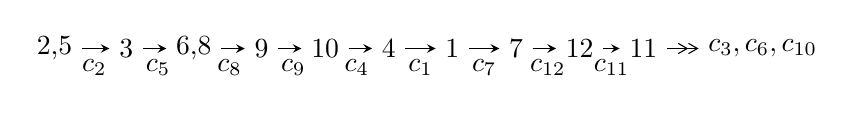
\begin{tikzpicture}[x=23pt, y=7pt]
	% node
	\node (A0) at (-1/8, 0) {2,5};
	\node (A1) at (1, 0) {3};
	\node (A2) at (33/16, 0) {6,8};
	\node (A3) at (25/8, 0) {9};
	\node (A4) at (33/8, 0) {10};
	\node (A5) at (41/8, 0) {4};
	\node (A6) at (49/8, 0) {1};
	\node (A7) at (57/8, 0) {7};
	\node (A8) at (65/8, 0) {12};
	\node (A9) at (73/8, 0) {11};
	\node (C1) at (1/2, -1) {$c_{2}$};
	\node (C2) at (3/2, -1) {$c_{5}$};
	\node (C3) at (21/8, -1) {$c_{8}$};
	\node (C4) at (29/8, -1) {$c_{9}$};
	\node (C5) at (37/8, -1) {$c_{4}$};
	\node (C6) at (45/8, -1) {$c_{1}$};
	\node (C7) at (53/8, -1) {$c_{7}$};
	\node (C8) at (61/8, -1) {$c_{12}$};
	\node (C9) at (69/8, -1) {$c_{11}$};
	\node (A10) at (11, 0) {$c_{3},c_{6},c_{10}$};

	% edge
	\draw[->,>=stealth]	
	(A0) edge (A1) (A1) edge (A2) (A2) edge (A3) (A3) edge (A4) (A4) edge (A5) (A5) edge (A6) (A6) edge (A7) (A7) edge (A8) (A8) edge (A9) ;
	\draw[->>,>={angle 60}]	
	(A9) edge (A10);
\end{tikzpicture} \\ 

\end{tabular} \\

\footnotetext{
The image of knot diagram is generated by the software ``\textbf{Draw programme}" developed by Andrew Bartholomew(\url{http://www.layer8.co.uk/maths/draw/index.htm\#Running-draw}), where we modified some parts for our purpose(\url{https://github.com/CATsTAILs/LinksPainter}).
}\phantom \\ \newline 
\centering \textbf{Ideals for irreducible components\footnotemark of $X_{\text{par}}$} 
 
\begin{align*}
I^u_{1}&=\langle 
257 u^{24}-3084 u^{23}+\cdots+64 b+37824,\;-77 u^{24}+410 u^{23}+\cdots+128 a+14912,\\
\phantom{I^u_{1}}&\phantom{= \langle  }u^{25}-12 u^{24}+\cdots+640 u-128\rangle \\
I^u_{2}&=\langle 
-10 a^5 u^2+16 a^4 u^2+\cdots-109 a+76,\\
\phantom{I^u_{2}}&\phantom{= \langle  }a^6- a^4 u^2-2 a^4 u-2 a^3 u^2-2 a^4-3 a^3 u+a^2 u^2- a^3+a^2 u+4 u^2 a- a^2+7 a u-3 u^2+4 a-4 u-2,\\
\phantom{I^u_{2}}&\phantom{= \langle  }u^3+u^2-1\rangle \\
I^u_{3}&=\langle 
2 u^{13}+7 u^{12}+u^{11}-26 u^{10}-32 u^9+24 u^8+74 u^7+23 u^6-63 u^5-51 u^4+16 u^3+26 u^2+b-5,\\
\phantom{I^u_{3}}&\phantom{= \langle  }5 u^{14}+17 u^{13}+\cdots+a-5,\\
\phantom{I^u_{3}}&\phantom{= \langle  }u^{15}+3 u^{14}- u^{13}-13 u^{12}-11 u^{11}+18 u^{10}+34 u^9- u^8-39 u^7-19 u^6+19 u^5+17 u^4-4 u^3-6 u^2+1\rangle \\
I^u_{4}&=\langle 
-44 a^7 u^2-73 a^6 u^2+\cdots-213 a+245,\;-2 a^6 u^2- a^5 u^2+\cdots+7 a+13,\;u^3+u^2-1\rangle \\
\\
\end{align*}
\raggedright * 4 irreducible components of $\dim_{\mathbb{C}}=0$, with total 82 representations.\\
\footnotetext{All coefficients of polynomials are rational numbers. But the coefficients are sometimes approximated in decimal forms when there is not enough margin.}
\newpage
\renewcommand{\arraystretch}{1}
\centering \section*{I. $I^u_{1}= \langle 257 u^{24}-3084 u^{23}+\cdots+64 b+37824,\;-77 u^{24}+410 u^{23}+\cdots+128 a+14912,\;u^{25}-12 u^{24}+\cdots+640 u-128 \rangle$}
\flushleft \textbf{(i) Arc colorings}\\
\begin{tabular}{m{7pt} m{180pt} m{7pt} m{180pt} }
\flushright $a_{2}=$&$\begin{pmatrix}1\\0\end{pmatrix}$ \\
\flushright $a_{5}=$&$\begin{pmatrix}0\\u\end{pmatrix}$ \\
\flushright $a_{3}=$&$\begin{pmatrix}1\\- u^2\end{pmatrix}$ \\
\flushright $a_{6}=$&$\begin{pmatrix}u\\- u^3+u\end{pmatrix}$ \\
\flushright $a_{8}=$&$\begin{pmatrix}\frac{77}{128} u^{24}-\frac{205}{64} u^{23}+\cdots+432 u-\frac{233}{2}\\-\frac{257}{64} u^{24}+\frac{771}{16} u^{23}+\cdots+\frac{4961}{2} u-591\end{pmatrix}$ \\
\flushright $a_{9}=$&$\begin{pmatrix}\frac{77}{128} u^{24}-\frac{205}{64} u^{23}+\cdots+432 u-\frac{233}{2}\\-\frac{853}{64} u^{24}+\frac{579}{4} u^{23}+\cdots+\frac{9947}{2} u-1105\end{pmatrix}$ \\
\flushright $a_{10}=$&$\begin{pmatrix}\frac{77}{128} u^{24}-\frac{801}{64} u^{23}+\cdots-1547 u+\frac{795}{2}\\\frac{715}{64} u^{24}-\frac{1849}{16} u^{23}+\cdots-\frac{5931}{2} u+601\end{pmatrix}$ \\
\flushright $a_{4}=$&$\begin{pmatrix}-\frac{1}{16} u^{24}+\frac{5}{8} u^{23}+\cdots+4 u+\frac{1}{2}\\-\frac{1}{8} u^{23}+\frac{5}{4} u^{22}+\cdots-\frac{63}{2} u+8\end{pmatrix}$ \\
\flushright $a_{1}=$&$\begin{pmatrix}-\frac{15}{16} u^{24}+\frac{167}{16} u^{23}+\cdots+\frac{1391}{4} u-71\\-\frac{15}{16} u^{24}+\frac{77}{8} u^{23}+\cdots+128 u-16\end{pmatrix}$ \\
\flushright $a_{7}=$&$\begin{pmatrix}\frac{65}{8} u^{24}-\frac{1579}{16} u^{23}+\cdots-5798 u+1396\\\frac{333}{16} u^{24}-\frac{3509}{16} u^{23}+\cdots-5955 u+1208\end{pmatrix}$ \\
\flushright $a_{12}=$&$\begin{pmatrix}-\frac{41}{16} u^{24}+\frac{455}{16} u^{23}+\cdots+\frac{3727}{4} u-191\\-\frac{41}{16} u^{24}+\frac{199}{8} u^{23}+\cdots-40 u+56\end{pmatrix}$ \\
\flushright $a_{11}=$&$\begin{pmatrix}-\frac{421}{64} u^{24}+\frac{4673}{64} u^{23}+\cdots+\frac{11579}{4} u-663\\-\frac{423}{64} u^{24}+\frac{1921}{32} u^{23}+\cdots+110 u+70\end{pmatrix}$\\&\end{tabular}
\flushleft \textbf{(ii) Obstruction class $= -1$}\\~\\
\flushleft \textbf{(iii) Cusp Shapes $= \frac{553}{16} u^{24}-\frac{3059}{8} u^{23}+\cdots-15300 u+3482$}\\~\\
\newpage\renewcommand{\arraystretch}{1}
\flushleft \textbf{(iv) u-Polynomials at the component}\newline \\
\begin{tabular}{m{50pt}|m{274pt}}
Crossings & \hspace{64pt}u-Polynomials at each crossing \\
\hline $$\begin{aligned}c_{1}\end{aligned}$$&$\begin{aligned}
&u^{25}-3 u^{24}+\cdots+2 u+1
\end{aligned}$\\
\hline $$\begin{aligned}c_{2},c_{5}\end{aligned}$$&$\begin{aligned}
&u^{25}+12 u^{24}+\cdots+640 u+128
\end{aligned}$\\
\hline $$\begin{aligned}c_{3},c_{4},c_{8}\\c_{10}\end{aligned}$$&$\begin{aligned}
&u^{25}- u^{24}+\cdots+2 u-1
\end{aligned}$\\
\hline $$\begin{aligned}c_{6},c_{11},c_{12}\end{aligned}$$&$\begin{aligned}
&u^{25}+6 u^{24}+\cdots+40 u+8
\end{aligned}$\\
\hline $$\begin{aligned}c_{7}\end{aligned}$$&$\begin{aligned}
&u^{25}-6 u^{24}+\cdots-56 u+464
\end{aligned}$\\
\hline $$\begin{aligned}c_{9}\end{aligned}$$&$\begin{aligned}
&u^{25}+u^{24}+\cdots-2 u+1
\end{aligned}$\\
\hline
\end{tabular}\\~\\
\newpage\renewcommand{\arraystretch}{1}
\flushleft \textbf{(v) Riley Polynomials at the component}\newline \\
\begin{tabular}{m{50pt}|m{274pt}}
Crossings & \hspace{64pt}Riley Polynomials at each crossing \\
\hline $$\begin{aligned}c_{1}\end{aligned}$$&$\begin{aligned}
&y^{25}-27 y^{24}+\cdots+54 y-1
\end{aligned}$\\
\hline $$\begin{aligned}c_{2},c_{5}\end{aligned}$$&$\begin{aligned}
&y^{25}-12 y^{24}+\cdots+114688 y-16384
\end{aligned}$\\
\hline $$\begin{aligned}c_{3},c_{4},c_{8}\\c_{10}\end{aligned}$$&$\begin{aligned}
&y^{25}-5 y^{24}+\cdots+18 y-1
\end{aligned}$\\
\hline $$\begin{aligned}c_{6},c_{11},c_{12}\end{aligned}$$&$\begin{aligned}
&y^{25}+22 y^{24}+\cdots+416 y-64
\end{aligned}$\\
\hline $$\begin{aligned}c_{7}\end{aligned}$$&$\begin{aligned}
&y^{25}-2 y^{24}+\cdots-995392 y-215296
\end{aligned}$\\
\hline $$\begin{aligned}c_{9}\end{aligned}$$&$\begin{aligned}
&y^{25}-23 y^{24}+\cdots+66 y-1
\end{aligned}$\\
\hline
\end{tabular}\\~\\
\newpage\flushleft \textbf{(vi) Complex Volumes and Cusp Shapes}
$$\begin{array}{c|c|c}  
\text{Solutions to }I^u_{1}& \I (\text{vol} + \sqrt{-1}CS) & \text{Cusp shape}\\
 \hline 
\begin{aligned}
u &= \phantom{-}0.439994 + 0.950507 I \\
a &= \phantom{-}0.449056 + 0.849462 I \\
b &= \phantom{-}0.905847 + 0.107899 I\end{aligned}
 & -3.00593 - 0.74051 I & \phantom{-}5.05508 + 0.18570 I \\ \hline\begin{aligned}
u &= \phantom{-}0.439994 - 0.950507 I \\
a &= \phantom{-}0.449056 - 0.849462 I \\
b &= \phantom{-}0.905847 - 0.107899 I\end{aligned}
 & -3.00593 + 0.74051 I & \phantom{-}5.05508 - 0.18570 I \\ \hline\begin{aligned}
u &= \phantom{-}0.617552 + 0.911770 I \\
a &= -0.520485 - 0.949952 I \\
b &= -1.202860 - 0.092876 I\end{aligned}
 & -9.79766 + 1.38415 I & \phantom{-}2.19427 - 0.69570 I \\ \hline\begin{aligned}
u &= \phantom{-}0.617552 - 0.911770 I \\
a &= -0.520485 + 0.949952 I \\
b &= -1.202860 + 0.092876 I\end{aligned}
 & -9.79766 - 1.38415 I & \phantom{-}2.19427 + 0.69570 I \\ \hline\begin{aligned}
u &= -0.155216 + 0.814496 I \\
a &= \phantom{-}0.569549 + 0.594113 I \\
b &= \phantom{-}0.482434 + 0.018405 I\end{aligned}
 & -2.49837 - 1.57308 I & \phantom{-}4.64082 + 4.61190 I \\ \hline\begin{aligned}
u &= -0.155216 - 0.814496 I \\
a &= \phantom{-}0.569549 - 0.594113 I \\
b &= \phantom{-}0.482434 - 0.018405 I\end{aligned}
 & -2.49837 + 1.57308 I & \phantom{-}4.64082 - 4.61190 I \\ \hline\begin{aligned}
u &= \phantom{-}0.473172 + 1.138930 I \\
a &= -0.327562 - 0.860505 I \\
b &= -0.840347 - 0.335702 I\end{aligned}
 & -1.79770 - 4.91771 I & \phantom{-}8.41927 + 6.28509 I \\ \hline\begin{aligned}
u &= \phantom{-}0.473172 - 1.138930 I \\
a &= -0.327562 + 0.860505 I \\
b &= -0.840347 + 0.335702 I\end{aligned}
 & -1.79770 + 4.91771 I & \phantom{-}8.41927 - 6.28509 I \\ \hline\begin{aligned}
u &= \phantom{-}1.097810 + 0.681530 I \\
a &= -0.926077 - 0.303192 I \\
b &= -1.55305 + 0.96565 I\end{aligned}
 & -8.25231 + 4.52896 I & \phantom{-}4.39857 - 4.77646 I \\ \hline\begin{aligned}
u &= \phantom{-}1.097810 - 0.681530 I \\
a &= -0.926077 + 0.303192 I \\
b &= -1.55305 - 0.96565 I\end{aligned}
 & -8.25231 - 4.52896 I & \phantom{-}4.39857 + 4.77646 I\\
 \hline 
 \end{array}$$\newpage$$\begin{array}{c|c|c}  
\text{Solutions to }I^u_{1}& \I (\text{vol} + \sqrt{-1}CS) & \text{Cusp shape}\\
 \hline 
\begin{aligned}
u &= \phantom{-}0.569528 + 1.179720 I \\
a &= \phantom{-}0.270690 + 0.922850 I \\
b &= \phantom{-}0.887146 + 0.468456 I\end{aligned}
 & -7.44241 - 8.72137 I & \phantom{-}5.19162 + 6.35185 I \\ \hline\begin{aligned}
u &= \phantom{-}0.569528 - 1.179720 I \\
a &= \phantom{-}0.270690 - 0.922850 I \\
b &= \phantom{-}0.887146 - 0.468456 I\end{aligned}
 & -7.44241 + 8.72137 I & \phantom{-}5.19162 - 6.35185 I \\ \hline\begin{aligned}
u &= \phantom{-}1.32152\phantom{ +0.000000I} \\
a &= -0.469575\phantom{ +0.000000I} \\
b &= -1.93007\phantom{ +0.000000I}\end{aligned}
 & \phantom{-}5.64216\phantom{ +0.000000I} & \phantom{-}30.1590\phantom{ +0.000000I} \\ \hline\begin{aligned}
u &= \phantom{-}1.306160 + 0.296832 I \\
a &= \phantom{-}0.548745 + 0.102029 I \\
b &= \phantom{-}1.63919 - 0.62194 I\end{aligned}
 & \phantom{-}1.99285 + 5.34908 I & \phantom{-}13.9471 - 13.2059 I \\ \hline\begin{aligned}
u &= \phantom{-}1.306160 - 0.296832 I \\
a &= \phantom{-}0.548745 - 0.102029 I \\
b &= \phantom{-}1.63919 + 0.62194 I\end{aligned}
 & \phantom{-}1.99285 - 5.34908 I & \phantom{-}13.9471 + 13.2059 I \\ \hline\begin{aligned}
u &= \phantom{-}1.214200 + 0.704239 I \\
a &= \phantom{-}0.907328 + 0.113165 I \\
b &= \phantom{-}1.41310 - 1.02138 I\end{aligned}
 & -0.61951 + 6.87942 I & \phantom{-}8.00000 - 4.38169 I \\ \hline\begin{aligned}
u &= \phantom{-}1.214200 - 0.704239 I \\
a &= \phantom{-}0.907328 - 0.113165 I \\
b &= \phantom{-}1.41310 + 1.02138 I\end{aligned}
 & -0.61951 - 6.87942 I & \phantom{-}8.00000 + 4.38169 I \\ \hline\begin{aligned}
u &= \phantom{-}1.22071 + 0.77249 I \\
a &= -0.990264 - 0.040589 I \\
b &= -1.37746 + 1.13069 I\end{aligned}
 & \phantom{-}0.51235 + 11.71780 I & \phantom{-}8.00000 - 8.48371 I \\ \hline\begin{aligned}
u &= \phantom{-}1.22071 - 0.77249 I \\
a &= -0.990264 + 0.040589 I \\
b &= -1.37746 - 1.13069 I\end{aligned}
 & \phantom{-}0.51235 - 11.71780 I & \phantom{-}8.00000 + 8.48371 I \\ \hline\begin{aligned}
u &= \phantom{-}1.20009 + 0.80742 I \\
a &= \phantom{-}1.066910 + 0.022071 I \\
b &= \phantom{-}1.40118 - 1.21648 I\end{aligned}
 & -5.4265 + 15.7509 I & \phantom{-}8.00000 - 8.57855 I\\
 \hline 
 \end{array}$$\newpage$$\begin{array}{c|c|c}  
\text{Solutions to }I^u_{1}& \I (\text{vol} + \sqrt{-1}CS) & \text{Cusp shape}\\
 \hline 
\begin{aligned}
u &= \phantom{-}1.20009 - 0.80742 I \\
a &= \phantom{-}1.066910 - 0.022071 I \\
b &= \phantom{-}1.40118 + 1.21648 I\end{aligned}
 & -5.4265 - 15.7509 I & \phantom{-}8.00000 + 8.57855 I \\ \hline\begin{aligned}
u &= -0.338292\phantom{ +0.000000I} \\
a &= -1.19055\phantom{ +0.000000I} \\
b &= -0.300946\phantom{ +0.000000I}\end{aligned}
 & \phantom{-}0.647725\phantom{ +0.000000I} & \phantom{-}15.2540\phantom{ +0.000000I} \\ \hline\begin{aligned}
u &= -1.66374\phantom{ +0.000000I} \\
a &= \phantom{-}0.444714\phantom{ +0.000000I} \\
b &= \phantom{-}0.277763\phantom{ +0.000000I}\end{aligned}
 & \phantom{-}6.10335\phantom{ +0.000000I} & \phantom{-}20.9380\phantom{ +0.000000I} \\ \hline\begin{aligned}
u &= -1.64375 + 0.30866 I \\
a &= -0.440186 - 0.060519 I \\
b &= -0.278561 - 0.018758 I\end{aligned}
 & \phantom{-}2.17466 - 4.23595 I & \phantom{-0.000000 } 0 \\ \hline\begin{aligned}
u &= -1.64375 - 0.30866 I \\
a &= -0.440186 + 0.060519 I \\
b &= -0.278561 + 0.018758 I\end{aligned}
 & \phantom{-}2.17466 + 4.23595 I & \phantom{-0.000000 } 0\\
 \hline 
 \end{array}$$\newpage\newpage\renewcommand{\arraystretch}{1}
\centering \section*{II. $I^u_{2}= \langle -10 a^5 u^2+16 a^4 u^2+\cdots-109 a+76,\;- a^4 u^2-2 a^3 u^2+\cdots+4 a-2,\;u^3+u^2-1 \rangle$}
\flushleft \textbf{(i) Arc colorings}\\
\begin{tabular}{m{7pt} m{180pt} m{7pt} m{180pt} }
\flushright $a_{2}=$&$\begin{pmatrix}1\\0\end{pmatrix}$ \\
\flushright $a_{5}=$&$\begin{pmatrix}0\\u\end{pmatrix}$ \\
\flushright $a_{3}=$&$\begin{pmatrix}1\\- u^2\end{pmatrix}$ \\
\flushright $a_{6}=$&$\begin{pmatrix}u\\u^2+u-1\end{pmatrix}$ \\
\flushright $a_{8}=$&$\begin{pmatrix}a\\0.169492 a^{5} u^{2}-0.271186 a^{4} u^{2}+\cdots+1.84746 a-1.28814\end{pmatrix}$ \\
\flushright $a_{9}=$&$\begin{pmatrix}a\\0.169492 a^{5} u^{2}-0.271186 a^{4} u^{2}+\cdots+1.84746 a-1.28814\end{pmatrix}$ \\
\flushright $a_{10}=$&$\begin{pmatrix}-0.135593 a^{5} u^{2}+0.0169492 a^{4} u^{2}+\cdots-0.677966 a+0.830508\\-0.457627 a^{5} u^{2}-0.0677966 a^{4} u^{2}+\cdots+0.711864 a-1.32203\end{pmatrix}$ \\
\flushright $a_{4}=$&$\begin{pmatrix}- a^2 u\\0.0677966 a^{5} u^{2}+0.491525 a^{4} u^{2}+\cdots-0.661017 a+1.08475\end{pmatrix}$ \\
\flushright $a_{1}=$&$\begin{pmatrix}0.203390 a^{5} u^{2}-0.525424 a^{4} u^{2}+\cdots+1.01695 a+1.25424\\0.610169 a^{5} u^{2}+0.423729 a^{4} u^{2}+\cdots+1.05085 a+0.762712\end{pmatrix}$ \\
\flushright $a_{7}=$&$\begin{pmatrix}-0.271186 a^{5} u^{2}+1.03390 a^{4} u^{2}+\cdots-1.35593 a+0.661017\\- a^5 u^2- a^3 u^2+\cdots- a^2+1\end{pmatrix}$ \\
\flushright $a_{12}=$&$\begin{pmatrix}0.0677966 a^{5} u^{2}-0.508475 a^{4} u^{2}+\cdots+0.338983 a+2.08475\\-0.0169492 a^{5} u^{2}+0.627119 a^{4} u^{2}+\cdots+0.915254 a+0.728814\end{pmatrix}$ \\
\flushright $a_{11}=$&$\begin{pmatrix}0.237288 a^{5} u^{2}+0.220339 a^{4} u^{2}+\cdots+1.18644 a-1.20339\\1.67797 a^{5} u^{2}-0.0847458 a^{4} u^{2}+\cdots+0.389831 a+0.847458\end{pmatrix}$\\&\end{tabular}
\flushleft \textbf{(ii) Obstruction class $= -1$}\\~\\
\flushleft \textbf{(iii) Cusp Shapes $= \frac{152}{59} a^5 u^2+\frac{40}{59} a^4 u^2+\cdots-\frac{184}{59} a+\frac{1134}{59}$}\\~\\
\newpage\renewcommand{\arraystretch}{1}
\flushleft \textbf{(iv) u-Polynomials at the component}\newline \\
\begin{tabular}{m{50pt}|m{274pt}}
Crossings & \hspace{64pt}u-Polynomials at each crossing \\
\hline $$\begin{aligned}c_{1}\end{aligned}$$&$\begin{aligned}
&u^{18}-2 u^{17}+\cdots-252 u-27
\end{aligned}$\\
\hline $$\begin{aligned}c_{2},c_{5}\end{aligned}$$&$\begin{aligned}
&(u^3- u^2+1)^6
\end{aligned}$\\
\hline $$\begin{aligned}c_{3},c_{4},c_{8}\\c_{10}\end{aligned}$$&$\begin{aligned}
&u^{18}-3 u^{16}+\cdots+6 u-11
\end{aligned}$\\
\hline $$\begin{aligned}c_{6},c_{11},c_{12}\end{aligned}$$&$\begin{aligned}
&(u^3+2 u+1)^6
\end{aligned}$\\
\hline $$\begin{aligned}c_{7}\end{aligned}$$&$\begin{aligned}
&(u^3+3 u^2+5 u+2)^6
\end{aligned}$\\
\hline $$\begin{aligned}c_{9}\end{aligned}$$&$\begin{aligned}
&u^{18}+u^{16}+\cdots-52 u-43
\end{aligned}$\\
\hline
\end{tabular}\\~\\
\newpage\renewcommand{\arraystretch}{1}
\flushleft \textbf{(v) Riley Polynomials at the component}\newline \\
\begin{tabular}{m{50pt}|m{274pt}}
Crossings & \hspace{64pt}Riley Polynomials at each crossing \\
\hline $$\begin{aligned}c_{1}\end{aligned}$$&$\begin{aligned}
&y^{18}-6 y^{17}+\cdots-81000 y+729
\end{aligned}$\\
\hline $$\begin{aligned}c_{2},c_{5}\end{aligned}$$&$\begin{aligned}
&(y^3- y^2+2 y-1)^6
\end{aligned}$\\
\hline $$\begin{aligned}c_{3},c_{4},c_{8}\\c_{10}\end{aligned}$$&$\begin{aligned}
&y^{18}-6 y^{17}+\cdots-1136 y+121
\end{aligned}$\\
\hline $$\begin{aligned}c_{6},c_{11},c_{12}\end{aligned}$$&$\begin{aligned}
&(y^3+4 y^2+4 y-1)^6
\end{aligned}$\\
\hline $$\begin{aligned}c_{7}\end{aligned}$$&$\begin{aligned}
&(y^3+y^2+13 y-4)^6
\end{aligned}$\\
\hline $$\begin{aligned}c_{9}\end{aligned}$$&$\begin{aligned}
&y^{18}+2 y^{17}+\cdots-17840 y+1849
\end{aligned}$\\
\hline
\end{tabular}\\~\\
\newpage\flushleft \textbf{(vi) Complex Volumes and Cusp Shapes}
$$\begin{array}{c|c|c}  
\text{Solutions to }I^u_{2}& \I (\text{vol} + \sqrt{-1}CS) & \text{Cusp shape}\\
 \hline 
\begin{aligned}
u &= -0.877439 + 0.744862 I \\
a &= -0.927224 - 0.015489 I \\
b &= -0.407238 - 0.969235 I\end{aligned}
 & \phantom{-}2.69787 - 2.82812 I & \phantom{-}17.1261 + 2.9794 I \\ \hline\begin{aligned}
u &= -0.877439 + 0.744862 I \\
a &= \phantom{-}1.104550 - 0.072177 I \\
b &= \phantom{-}1.63644 + 0.28753 I\end{aligned}
 & -7.53006 + 2.30982 I & \phantom{-}5.17231 - 0.22957 I \\ \hline\begin{aligned}
u &= -0.877439 + 0.744862 I \\
a &= \phantom{-}0.187603 + 1.191150 I \\
b &= -0.734633 + 0.080557 I\end{aligned}
 & -7.53006 + 2.30982 I & \phantom{-}5.17231 - 0.22957 I \\ \hline\begin{aligned}
u &= -0.877439 + 0.744862 I \\
a &= -1.241110 - 0.215785 I \\
b &= -1.66753 - 0.94699 I\end{aligned}
 & -7.53006 - 7.96606 I & \phantom{-}5.17231 + 6.18847 I \\ \hline\begin{aligned}
u &= -0.877439 + 0.744862 I \\
a &= \phantom{-}0.346778 - 1.240900 I \\
b &= \phantom{-}0.918807 + 0.323963 I\end{aligned}
 & -7.53006 - 7.96606 I & \phantom{-}5.17231 + 6.18847 I \\ \hline\begin{aligned}
u &= -0.877439 + 0.744862 I \\
a &= \phantom{-}0.529395 + 0.353208 I \\
b &= \phantom{-}0.254152 + 1.224170 I\end{aligned}
 & \phantom{-}2.69787 - 2.82812 I & \phantom{-}17.1261 + 2.9794 I \\ \hline\begin{aligned}
u &= -0.877439 - 0.744862 I \\
a &= -0.927224 + 0.015489 I \\
b &= -0.407238 + 0.969235 I\end{aligned}
 & \phantom{-}2.69787 + 2.82812 I & \phantom{-}17.1261 - 2.9794 I \\ \hline\begin{aligned}
u &= -0.877439 - 0.744862 I \\
a &= \phantom{-}1.104550 + 0.072177 I \\
b &= \phantom{-}1.63644 - 0.28753 I\end{aligned}
 & -7.53006 - 2.30982 I & \phantom{-}5.17231 + 0.22957 I \\ \hline\begin{aligned}
u &= -0.877439 - 0.744862 I \\
a &= \phantom{-}0.187603 - 1.191150 I \\
b &= -0.734633 - 0.080557 I\end{aligned}
 & -7.53006 - 2.30982 I & \phantom{-}5.17231 + 0.22957 I \\ \hline\begin{aligned}
u &= -0.877439 - 0.744862 I \\
a &= -1.241110 + 0.215785 I \\
b &= -1.66753 + 0.94699 I\end{aligned}
 & -7.53006 + 7.96606 I & \phantom{-}5.17231 - 6.18847 I\\
 \hline 
 \end{array}$$\newpage$$\begin{array}{c|c|c}  
\text{Solutions to }I^u_{2}& \I (\text{vol} + \sqrt{-1}CS) & \text{Cusp shape}\\
 \hline 
\begin{aligned}
u &= -0.877439 - 0.744862 I \\
a &= \phantom{-}0.346778 + 1.240900 I \\
b &= \phantom{-}0.918807 - 0.323963 I\end{aligned}
 & -7.53006 + 7.96606 I & \phantom{-}5.17231 - 6.18847 I \\ \hline\begin{aligned}
u &= -0.877439 - 0.744862 I \\
a &= \phantom{-}0.529395 - 0.353208 I \\
b &= \phantom{-}0.254152 - 1.224170 I\end{aligned}
 & \phantom{-}2.69787 + 2.82812 I & \phantom{-}17.1261 - 2.9794 I \\ \hline\begin{aligned}
u &= \phantom{-}0.754878\phantom{ +0.000000I} \\
a &= \phantom{-}0.737750 + 0.212805 I \\
b &= \phantom{-}0.61766 + 2.03584 I\end{aligned}
 & -3.39248 + 5.13794 I & \phantom{-}11.70158 - 3.20902 I \\ \hline\begin{aligned}
u &= \phantom{-}0.754878\phantom{ +0.000000I} \\
a &= \phantom{-}0.737750 - 0.212805 I \\
b &= \phantom{-}0.61766 - 2.03584 I\end{aligned}
 & -3.39248 - 5.13794 I & \phantom{-}11.70158 + 3.20902 I \\ \hline\begin{aligned}
u &= \phantom{-}0.754878\phantom{ +0.000000I} \\
a &= -0.90888 + 1.32075 I \\
b &= -0.090652 - 1.376170 I\end{aligned}
 & -3.39248 - 5.13794 I & \phantom{-}11.70158 + 3.20902 I \\ \hline\begin{aligned}
u &= \phantom{-}0.754878\phantom{ +0.000000I} \\
a &= -0.90888 - 1.32075 I \\
b &= -0.090652 + 1.376170 I\end{aligned}
 & -3.39248 + 5.13794 I & \phantom{-}11.70158 - 3.20902 I \\ \hline\begin{aligned}
u &= \phantom{-}0.754878\phantom{ +0.000000I} \\
a &= -1.94302\phantom{ +0.000000I} \\
b &= -1.43643\phantom{ +0.000000I}\end{aligned}
 & \phantom{-}6.83546\phantom{ +0.000000I} & \phantom{-}23.6550\phantom{ +0.000000I} \\ \hline\begin{aligned}
u &= \phantom{-}0.754878\phantom{ +0.000000I} \\
a &= \phantom{-}2.28528\phantom{ +0.000000I} \\
b &= \phantom{-}0.382411\phantom{ +0.000000I}\end{aligned}
 & \phantom{-}6.83546\phantom{ +0.000000I} & \phantom{-}23.6550\phantom{ +0.000000I}\\
 \hline 
 \end{array}$$\newpage\newpage\renewcommand{\arraystretch}{1}
\centering \section*{III. $I^u_{3}= \langle 2 u^{13}+7 u^{12}+\cdots+b-5,\;5 u^{14}+17 u^{13}+\cdots+a-5,\;u^{15}+3 u^{14}+\cdots-6 u^2+1 \rangle$}
\flushleft \textbf{(i) Arc colorings}\\
\begin{tabular}{m{7pt} m{180pt} m{7pt} m{180pt} }
\flushright $a_{2}=$&$\begin{pmatrix}1\\0\end{pmatrix}$ \\
\flushright $a_{5}=$&$\begin{pmatrix}0\\u\end{pmatrix}$ \\
\flushright $a_{3}=$&$\begin{pmatrix}1\\- u^2\end{pmatrix}$ \\
\flushright $a_{6}=$&$\begin{pmatrix}u\\- u^3+u\end{pmatrix}$ \\
\flushright $a_{8}=$&$\begin{pmatrix}-5 u^{14}-17 u^{13}+\cdots+4 u+5\\-2 u^{13}-7 u^{12}+\cdots-26 u^2+5\end{pmatrix}$ \\
\flushright $a_{9}=$&$\begin{pmatrix}-5 u^{14}-17 u^{13}+\cdots+4 u+5\\3 u^{14}+8 u^{13}+\cdots-5 u+3\end{pmatrix}$ \\
\flushright $a_{10}=$&$\begin{pmatrix}-7 u^{14}-24 u^{13}+\cdots+9 u+5\\u^{14}+2 u^{13}+\cdots-2 u+2\end{pmatrix}$ \\
\flushright $a_{4}=$&$\begin{pmatrix}u^{14}+4 u^{13}+\cdots-10 u-6\\u^{14}+3 u^{13}+\cdots-4 u^2-5 u\end{pmatrix}$ \\
\flushright $a_{1}=$&$\begin{pmatrix}5 u^{14}+16 u^{13}+\cdots-17 u-8\\u^{13}+3 u^{12}+\cdots-4 u-4\end{pmatrix}$ \\
\flushright $a_{7}=$&$\begin{pmatrix}-9 u^{14}-32 u^{13}+\cdots+15 u+15\\-4 u^{14}-14 u^{13}+\cdots+10 u+3\end{pmatrix}$ \\
\flushright $a_{12}=$&$\begin{pmatrix}6 u^{14}+19 u^{13}+\cdots-21 u-8\\u^{14}+4 u^{13}+\cdots-7 u-4\end{pmatrix}$ \\
\flushright $a_{11}=$&$\begin{pmatrix}3 u^{14}+13 u^{13}+\cdots-3 u-4\\3 u^{14}+9 u^{13}+\cdots- u-1\end{pmatrix}$\\&\end{tabular}
\flushleft \textbf{(ii) Obstruction class $= 1$}\\~\\
\flushleft \textbf{(iii) Cusp Shapes $= 8 u^{14}+21 u^{13}-11 u^{12}-84 u^{11}-54 u^{10}+113 u^9+166 u^8-35 u^7-173 u^6-38 u^5+82 u^4+34 u^3-32 u^2-6 u+9$}\\~\\
\newpage\renewcommand{\arraystretch}{1}
\flushleft \textbf{(iv) u-Polynomials at the component}\newline \\
\begin{tabular}{m{50pt}|m{274pt}}
Crossings & \hspace{64pt}u-Polynomials at each crossing \\
\hline $$\begin{aligned}c_{1}\end{aligned}$$&$\begin{aligned}
&u^{15}+3 u^{14}+\cdots+4 u^2-1
\end{aligned}$\\
\hline $$\begin{aligned}c_{2}\end{aligned}$$&$\begin{aligned}
&u^{15}+3 u^{14}+\cdots-6 u^2+1
\end{aligned}$\\
\hline $$\begin{aligned}c_{3},c_{8}\end{aligned}$$&$\begin{aligned}
&u^{15}+u^{14}+\cdots+6 u^2-1
\end{aligned}$\\
\hline $$\begin{aligned}c_{4},c_{10}\end{aligned}$$&$\begin{aligned}
&u^{15}- u^{14}+\cdots-6 u^2+1
\end{aligned}$\\
\hline $$\begin{aligned}c_{5}\end{aligned}$$&$\begin{aligned}
&u^{15}-3 u^{14}+\cdots+6 u^2-1
\end{aligned}$\\
\hline $$\begin{aligned}c_{6}\end{aligned}$$&$\begin{aligned}
&u^{15}+u^{14}+\cdots-3 u^2+1
\end{aligned}$\\
\hline $$\begin{aligned}c_{7}\end{aligned}$$&$\begin{aligned}
&u^{15}- u^{14}+\cdots-2 u+1
\end{aligned}$\\
\hline $$\begin{aligned}c_{9}\end{aligned}$$&$\begin{aligned}
&u^{15}+u^{14}+\cdots-4 u^2+1
\end{aligned}$\\
\hline $$\begin{aligned}c_{11},c_{12}\end{aligned}$$&$\begin{aligned}
&u^{15}- u^{14}+\cdots+3 u^2-1
\end{aligned}$\\
\hline
\end{tabular}\\~\\
\newpage\renewcommand{\arraystretch}{1}
\flushleft \textbf{(v) Riley Polynomials at the component}\newline \\
\begin{tabular}{m{50pt}|m{274pt}}
Crossings & \hspace{64pt}Riley Polynomials at each crossing \\
\hline $$\begin{aligned}c_{1}\end{aligned}$$&$\begin{aligned}
&y^{15}+7 y^{14}+\cdots+8 y-1
\end{aligned}$\\
\hline $$\begin{aligned}c_{2},c_{5}\end{aligned}$$&$\begin{aligned}
&y^{15}-11 y^{14}+\cdots+12 y-1
\end{aligned}$\\
\hline $$\begin{aligned}c_{3},c_{4},c_{8}\\c_{10}\end{aligned}$$&$\begin{aligned}
&y^{15}-15 y^{14}+\cdots+12 y-1
\end{aligned}$\\
\hline $$\begin{aligned}c_{6},c_{11},c_{12}\end{aligned}$$&$\begin{aligned}
&y^{15}+15 y^{14}+\cdots+6 y-1
\end{aligned}$\\
\hline $$\begin{aligned}c_{7}\end{aligned}$$&$\begin{aligned}
&y^{15}-5 y^{14}+\cdots+2 y-1
\end{aligned}$\\
\hline $$\begin{aligned}c_{9}\end{aligned}$$&$\begin{aligned}
&y^{15}+3 y^{14}+\cdots+8 y-1
\end{aligned}$\\
\hline
\end{tabular}\\~\\
\newpage\flushleft \textbf{(vi) Complex Volumes and Cusp Shapes}
$$\begin{array}{c|c|c}  
\text{Solutions to }I^u_{3}& \I (\text{vol} + \sqrt{-1}CS) & \text{Cusp shape}\\
 \hline 
\begin{aligned}
u &= -0.772963 + 0.597189 I \\
a &= -0.827811 - 0.016279 I \\
b &= -0.343553 - 1.218360 I\end{aligned}
 & \phantom{-}1.77519 - 3.34740 I & \phantom{-}8.50075 + 8.05329 I \\ \hline\begin{aligned}
u &= -0.772963 - 0.597189 I \\
a &= -0.827811 + 0.016279 I \\
b &= -0.343553 + 1.218360 I\end{aligned}
 & \phantom{-}1.77519 + 3.34740 I & \phantom{-}8.50075 - 8.05329 I \\ \hline\begin{aligned}
u &= \phantom{-}1.21630\phantom{ +0.000000I} \\
a &= -1.10982\phantom{ +0.000000I} \\
b &= -0.609066\phantom{ +0.000000I}\end{aligned}
 & \phantom{-}8.60341\phantom{ +0.000000I} & \phantom{-}19.2250\phantom{ +0.000000I} \\ \hline\begin{aligned}
u &= \phantom{-}1.216020 + 0.268411 I \\
a &= \phantom{-}1.037430 - 0.282211 I \\
b &= \phantom{-}0.591253 - 0.100818 I\end{aligned}
 & \phantom{-}4.59696 + 3.78442 I & \phantom{-}13.45506 - 3.52568 I \\ \hline\begin{aligned}
u &= \phantom{-}1.216020 - 0.268411 I \\
a &= \phantom{-}1.037430 + 0.282211 I \\
b &= \phantom{-}0.591253 + 0.100818 I\end{aligned}
 & \phantom{-}4.59696 - 3.78442 I & \phantom{-}13.45506 + 3.52568 I \\ \hline\begin{aligned}
u &= -0.741693 + 1.001970 I \\
a &= \phantom{-}0.645240 + 0.343179 I \\
b &= \phantom{-}0.168411 + 0.864224 I\end{aligned}
 & -1.02527 - 2.06106 I & \phantom{-}10.76904 + 5.89866 I \\ \hline\begin{aligned}
u &= -0.741693 - 1.001970 I \\
a &= \phantom{-}0.645240 - 0.343179 I \\
b &= \phantom{-}0.168411 - 0.864224 I\end{aligned}
 & -1.02527 + 2.06106 I & \phantom{-}10.76904 - 5.89866 I \\ \hline\begin{aligned}
u &= -0.581097 + 0.353670 I \\
a &= \phantom{-}1.215450 - 0.514042 I \\
b &= \phantom{-}0.12631 + 1.63261 I\end{aligned}
 & -4.31889 - 5.65349 I & \phantom{-}3.28441 + 7.61935 I \\ \hline\begin{aligned}
u &= -0.581097 - 0.353670 I \\
a &= \phantom{-}1.215450 + 0.514042 I \\
b &= \phantom{-}0.12631 - 1.63261 I\end{aligned}
 & -4.31889 + 5.65349 I & \phantom{-}3.28441 - 7.61935 I \\ \hline\begin{aligned}
u &= \phantom{-}0.661672\phantom{ +0.000000I} \\
a &= \phantom{-}2.39502\phantom{ +0.000000I} \\
b &= \phantom{-}0.953687\phantom{ +0.000000I}\end{aligned}
 & \phantom{-}6.37007\phantom{ +0.000000I} & \phantom{-}2.43460\phantom{ +0.000000I}\\
 \hline 
 \end{array}$$\newpage$$\begin{array}{c|c|c}  
\text{Solutions to }I^u_{3}& \I (\text{vol} + \sqrt{-1}CS) & \text{Cusp shape}\\
 \hline 
\begin{aligned}
u &= \phantom{-}0.577868 + 0.178736 I \\
a &= -2.47388 + 1.02720 I \\
b &= -0.998690 + 0.209089 I\end{aligned}
 & \phantom{-}1.98344 - 1.67719 I & \phantom{-}4.13214 - 1.25424 I \\ \hline\begin{aligned}
u &= \phantom{-}0.577868 - 0.178736 I \\
a &= -2.47388 - 1.02720 I \\
b &= -0.998690 - 0.209089 I\end{aligned}
 & \phantom{-}1.98344 + 1.67719 I & \phantom{-}4.13214 + 1.25424 I \\ \hline\begin{aligned}
u &= -1.41521\phantom{ +0.000000I} \\
a &= \phantom{-}0.382739\phantom{ +0.000000I} \\
b &= \phantom{-}1.30454\phantom{ +0.000000I}\end{aligned}
 & \phantom{-}5.30168\phantom{ +0.000000I} & \phantom{-}4.34420\phantom{ +0.000000I} \\ \hline\begin{aligned}
u &= -1.42952 + 0.46018 I \\
a &= -0.430407 - 0.024659 I \\
b &= -0.868313 - 0.551235 I\end{aligned}
 & \phantom{-}1.65539 - 4.71343 I & \phantom{-}7.35653 + 5.31534 I \\ \hline\begin{aligned}
u &= -1.42952 - 0.46018 I \\
a &= -0.430407 + 0.024659 I \\
b &= -0.868313 + 0.551235 I\end{aligned}
 & \phantom{-}1.65539 + 4.71343 I & \phantom{-}7.35653 - 5.31534 I\\
 \hline 
 \end{array}$$\newpage\newpage\renewcommand{\arraystretch}{1}
\centering \section*{IV. $I^u_{4}= \langle -44 a^7 u^2-73 a^6 u^2+\cdots-213 a+245,\;-2 a^6 u^2- a^5 u^2+\cdots+7 a+13,\;u^3+u^2-1 \rangle$}
\flushleft \textbf{(i) Arc colorings}\\
\begin{tabular}{m{7pt} m{180pt} m{7pt} m{180pt} }
\flushright $a_{2}=$&$\begin{pmatrix}1\\0\end{pmatrix}$ \\
\flushright $a_{5}=$&$\begin{pmatrix}0\\u\end{pmatrix}$ \\
\flushright $a_{3}=$&$\begin{pmatrix}1\\- u^2\end{pmatrix}$ \\
\flushright $a_{6}=$&$\begin{pmatrix}u\\u^2+u-1\end{pmatrix}$ \\
\flushright $a_{8}=$&$\begin{pmatrix}a\\0.273292 a^{7} u^{2}+0.453416 a^{6} u^{2}+\cdots+1.32298 a-1.52174\end{pmatrix}$ \\
\flushright $a_{9}=$&$\begin{pmatrix}a\\0.273292 a^{7} u^{2}+0.453416 a^{6} u^{2}+\cdots+1.32298 a-1.52174\end{pmatrix}$ \\
\flushright $a_{10}=$&$\begin{pmatrix}-0.677019 a^{7} u^{2}-0.645963 a^{6} u^{2}+\cdots+0.745342 a+1.56522\\-0.658385 a^{7} u^{2}-0.683230 a^{6} u^{2}+\cdots+1.40373 a-0.652174\end{pmatrix}$ \\
\flushright $a_{4}=$&$\begin{pmatrix}- a^2 u\\1.36025 a^{7} u^{2}+0.279503 a^{6} u^{2}+\cdots+0.0621118 a-0.869565\end{pmatrix}$ \\
\flushright $a_{1}=$&$\begin{pmatrix}-1.02484 a^{7} u^{2}-1.95031 a^{6} u^{2}+\cdots+2.78882 a+0.956522\\-1.16149 a^{7} u^{2}-0.677019 a^{6} u^{2}+\cdots-0.372671 a+1.21739\end{pmatrix}$ \\
\flushright $a_{7}=$&$\begin{pmatrix}-1.72671 a^{7} u^{2}-2.54658 a^{6} u^{2}+\cdots+5.32298 a+2.47826\\0.00621118 a^{7} u^{2}-2.01242 a^{6} u^{2}+\cdots+2.55280 a-1.73913\end{pmatrix}$ \\
\flushright $a_{12}=$&$\begin{pmatrix}0.608696 a^{7} u^{2}-2.21739 a^{6} u^{2}+\cdots+3.17391 a-0.434783\\-\frac{15}{7} a^7 u^2-\frac{5}{7} a^6 u^2+\cdots+\frac{9}{7} a+1\end{pmatrix}$ \\
\flushright $a_{11}=$&$\begin{pmatrix}-0.950311 a^{7} u^{2}+1.90062 a^{6} u^{2}+\cdots-2.57764 a-2.91304\\0.124224 a^{7} u^{2}+3.75155 a^{6} u^{2}+\cdots-4.94410 a-0.782609\end{pmatrix}$\\&\end{tabular}
\flushleft \textbf{(ii) Obstruction class $= -1$}\\~\\
\flushleft \textbf{(iii) Cusp Shapes $= -\frac{52}{23} a^7 u^2-\frac{80}{23} a^6 u^2+\cdots+\frac{248}{23} a+\frac{254}{23}$}\\~\\
\newpage\renewcommand{\arraystretch}{1}
\flushleft \textbf{(iv) u-Polynomials at the component}\newline \\
\begin{tabular}{m{50pt}|m{274pt}}
Crossings & \hspace{64pt}u-Polynomials at each crossing \\
\hline $$\begin{aligned}c_{1}\end{aligned}$$&$\begin{aligned}
&u^{24}-5 u^{23}+\cdots-20 u+109
\end{aligned}$\\
\hline $$\begin{aligned}c_{2},c_{5}\end{aligned}$$&$\begin{aligned}
&(u^3- u^2+1)^8
\end{aligned}$\\
\hline $$\begin{aligned}c_{3},c_{4},c_{8}\\c_{10}\end{aligned}$$&$\begin{aligned}
&u^{24}+u^{23}+\cdots-24 u+7
\end{aligned}$\\
\hline $$\begin{aligned}c_{6},c_{11},c_{12}\end{aligned}$$&$\begin{aligned}
&(u^4- u^3+2 u^2-2 u+1)^6
\end{aligned}$\\
\hline $$\begin{aligned}c_{7}\end{aligned}$$&$\begin{aligned}
&(u^2- u+1)^{12}
\end{aligned}$\\
\hline $$\begin{aligned}c_{9}\end{aligned}$$&$\begin{aligned}
&u^{24}+3 u^{23}+\cdots+20 u+19
\end{aligned}$\\
\hline
\end{tabular}\\~\\
\newpage\renewcommand{\arraystretch}{1}
\flushleft \textbf{(v) Riley Polynomials at the component}\newline \\
\begin{tabular}{m{50pt}|m{274pt}}
Crossings & \hspace{64pt}Riley Polynomials at each crossing \\
\hline $$\begin{aligned}c_{1}\end{aligned}$$&$\begin{aligned}
&y^{24}+9 y^{23}+\cdots+27504 y+11881
\end{aligned}$\\
\hline $$\begin{aligned}c_{2},c_{5}\end{aligned}$$&$\begin{aligned}
&(y^3- y^2+2 y-1)^8
\end{aligned}$\\
\hline $$\begin{aligned}c_{3},c_{4},c_{8}\\c_{10}\end{aligned}$$&$\begin{aligned}
&y^{24}-15 y^{23}+\cdots-716 y+49
\end{aligned}$\\
\hline $$\begin{aligned}c_{6},c_{11},c_{12}\end{aligned}$$&$\begin{aligned}
&(y^4+3 y^3+2 y^2+1)^6
\end{aligned}$\\
\hline $$\begin{aligned}c_{7}\end{aligned}$$&$\begin{aligned}
&(y^2+y+1)^{12}
\end{aligned}$\\
\hline $$\begin{aligned}c_{9}\end{aligned}$$&$\begin{aligned}
&y^{24}+5 y^{23}+\cdots+1424 y+361
\end{aligned}$\\
\hline
\end{tabular}\\~\\
\newpage\flushleft \textbf{(vi) Complex Volumes and Cusp Shapes}
$$\begin{array}{c|c|c}  
\text{Solutions to }I^u_{4}& \I (\text{vol} + \sqrt{-1}CS) & \text{Cusp shape}\\
 \hline 
\begin{aligned}
u &= -0.877439 + 0.744862 I \\
a &= -0.040773 - 0.997477 I \\
b &= \phantom{-}0.617792 + 0.097671 I\end{aligned}
 & -1.37919 - 0.79824 I & \phantom{-}8.49024 - 0.48465 I \\ \hline\begin{aligned}
u &= -0.877439 + 0.744862 I \\
a &= \phantom{-}0.964624 - 0.327636 I \\
b &= \phantom{-}0.525863 + 0.945972 I\end{aligned}
 & -1.37919 - 4.85801 I & \phantom{-}8.49024 + 6.44355 I \\ \hline\begin{aligned}
u &= -0.877439 + 0.744862 I \\
a &= -1.039300 - 0.058321 I \\
b &= -1.39358 - 0.47039 I\end{aligned}
 & -1.37919 - 0.79824 I & \phantom{-}8.49024 - 0.48465 I \\ \hline\begin{aligned}
u &= -0.877439 + 0.744862 I \\
a &= \phantom{-}1.033460 + 0.263154 I \\
b &= \phantom{-}0.303126 + 0.916009 I\end{aligned}
 & -1.37919 - 0.79824 I & \phantom{-}8.49024 - 0.48465 I \\ \hline\begin{aligned}
u &= -0.877439 + 0.744862 I \\
a &= -0.254667 + 1.040960 I \\
b &= -0.745244 - 0.312818 I\end{aligned}
 & -1.37919 - 4.85801 I & \phantom{-}8.49024 + 6.44355 I \\ \hline\begin{aligned}
u &= -0.877439 + 0.744862 I \\
a &= -0.747266 - 0.522075 I \\
b &= -0.56367 - 1.44433 I\end{aligned}
 & -1.37919 - 4.85801 I & \phantom{-}8.49024 + 6.44355 I \\ \hline\begin{aligned}
u &= -0.877439 + 0.744862 I \\
a &= \phantom{-}1.121100 + 0.196208 I \\
b &= \phantom{-}1.43883 + 0.82244 I\end{aligned}
 & -1.37919 - 4.85801 I & \phantom{-}8.49024 + 6.44355 I \\ \hline\begin{aligned}
u &= -0.877439 + 0.744862 I \\
a &= -0.159736 - 0.339671 I \\
b &= \phantom{-}0.154539 - 1.116840 I\end{aligned}
 & -1.37919 - 0.79824 I & \phantom{-}8.49024 - 0.48465 I \\ \hline\begin{aligned}
u &= -0.877439 - 0.744862 I \\
a &= -0.040773 + 0.997477 I \\
b &= \phantom{-}0.617792 - 0.097671 I\end{aligned}
 & -1.37919 + 0.79824 I & \phantom{-}8.49024 + 0.48465 I \\ \hline\begin{aligned}
u &= -0.877439 - 0.744862 I \\
a &= \phantom{-}0.964624 + 0.327636 I \\
b &= \phantom{-}0.525863 - 0.945972 I\end{aligned}
 & -1.37919 + 4.85801 I & \phantom{-}8.49024 - 6.44355 I\\
 \hline 
 \end{array}$$\newpage$$\begin{array}{c|c|c}  
\text{Solutions to }I^u_{4}& \I (\text{vol} + \sqrt{-1}CS) & \text{Cusp shape}\\
 \hline 
\begin{aligned}
u &= -0.877439 - 0.744862 I \\
a &= -1.039300 + 0.058321 I \\
b &= -1.39358 + 0.47039 I\end{aligned}
 & -1.37919 + 0.79824 I & \phantom{-}8.49024 + 0.48465 I \\ \hline\begin{aligned}
u &= -0.877439 - 0.744862 I \\
a &= \phantom{-}1.033460 - 0.263154 I \\
b &= \phantom{-}0.303126 - 0.916009 I\end{aligned}
 & -1.37919 + 0.79824 I & \phantom{-}8.49024 + 0.48465 I \\ \hline\begin{aligned}
u &= -0.877439 - 0.744862 I \\
a &= -0.254667 - 1.040960 I \\
b &= -0.745244 + 0.312818 I\end{aligned}
 & -1.37919 + 4.85801 I & \phantom{-}8.49024 - 6.44355 I \\ \hline\begin{aligned}
u &= -0.877439 - 0.744862 I \\
a &= -0.747266 + 0.522075 I \\
b &= -0.56367 + 1.44433 I\end{aligned}
 & -1.37919 + 4.85801 I & \phantom{-}8.49024 - 6.44355 I \\ \hline\begin{aligned}
u &= -0.877439 - 0.744862 I \\
a &= \phantom{-}1.121100 - 0.196208 I \\
b &= \phantom{-}1.43883 - 0.82244 I\end{aligned}
 & -1.37919 + 4.85801 I & \phantom{-}8.49024 - 6.44355 I \\ \hline\begin{aligned}
u &= -0.877439 - 0.744862 I \\
a &= -0.159736 + 0.339671 I \\
b &= \phantom{-}0.154539 + 1.116840 I\end{aligned}
 & -1.37919 + 0.79824 I & \phantom{-}8.49024 + 0.48465 I \\ \hline\begin{aligned}
u &= \phantom{-}0.754878\phantom{ +0.000000I} \\
a &= -0.935402 + 0.185618 I \\
b &= -0.56365 - 1.65106 I\end{aligned}
 & \phantom{-}2.75839 + 2.02988 I & \phantom{-}15.0195 - 3.4641 I \\ \hline\begin{aligned}
u &= \phantom{-}0.754878\phantom{ +0.000000I} \\
a &= -0.935402 - 0.185618 I \\
b &= -0.56365 + 1.65106 I\end{aligned}
 & \phantom{-}2.75839 - 2.02988 I & \phantom{-}15.0195 + 3.4641 I \\ \hline\begin{aligned}
u &= \phantom{-}0.754878\phantom{ +0.000000I} \\
a &= \phantom{-}1.027300 + 0.800722 I \\
b &= \phantom{-}0.28063 - 1.38647 I\end{aligned}
 & \phantom{-}2.75839 + 2.02988 I & \phantom{-}15.0195 - 3.4641 I \\ \hline\begin{aligned}
u &= \phantom{-}0.754878\phantom{ +0.000000I} \\
a &= \phantom{-}1.027300 - 0.800722 I \\
b &= \phantom{-}0.28063 + 1.38647 I\end{aligned}
 & \phantom{-}2.75839 - 2.02988 I & \phantom{-}15.0195 + 3.4641 I\\
 \hline 
 \end{array}$$\newpage$$\begin{array}{c|c|c}  
\text{Solutions to }I^u_{4}& \I (\text{vol} + \sqrt{-1}CS) & \text{Cusp shape}\\
 \hline 
\begin{aligned}
u &= \phantom{-}0.754878\phantom{ +0.000000I} \\
a &= \phantom{-}1.88775 + 0.07859 I \\
b &= \phantom{-}1.63567 + 0.61747 I\end{aligned}
 & \phantom{-}2.75839 + 2.02988 I & \phantom{-}15.0195 - 3.4641 I \\ \hline\begin{aligned}
u &= \phantom{-}0.754878\phantom{ +0.000000I} \\
a &= \phantom{-}1.88775 - 0.07859 I \\
b &= \phantom{-}1.63567 - 0.61747 I\end{aligned}
 & \phantom{-}2.75839 - 2.02988 I & \phantom{-}15.0195 + 3.4641 I \\ \hline\begin{aligned}
u &= \phantom{-}0.754878\phantom{ +0.000000I} \\
a &= -2.35710 + 0.41119 I \\
b &= -0.190292 - 0.406791 I\end{aligned}
 & \phantom{-}2.75839 - 2.02988 I & \phantom{-}15.0195 + 3.4641 I \\ \hline\begin{aligned}
u &= \phantom{-}0.754878\phantom{ +0.000000I} \\
a &= -2.35710 - 0.41119 I \\
b &= -0.190292 + 0.406791 I\end{aligned}
 & \phantom{-}2.75839 + 2.02988 I & \phantom{-}15.0195 - 3.4641 I\\
 \hline 
 \end{array}$$\newpage
\newpage\renewcommand{\arraystretch}{1}
\centering \section*{ V. u-Polynomials}
\begin{tabular}{m{50pt}|m{274pt}}
Crossings & \hspace{64pt}u-Polynomials at each crossing \\
\hline $$\begin{aligned}c_{1}\end{aligned}$$&$\begin{aligned}
&(u^{15}+3 u^{14}+\cdots+4 u^2-1)(u^{18}-2 u^{17}+\cdots-252 u-27)\\
&\cdot(u^{24}-5 u^{23}+\cdots-20 u+109)(u^{25}-3 u^{24}+\cdots+2 u+1)
\end{aligned}$\\
\hline $$\begin{aligned}c_{2}\end{aligned}$$&$\begin{aligned}
&((u^3- u^2+1)^{14})(u^{15}+3 u^{14}+\cdots-6 u^2+1)\\
&\cdot(u^{25}+12 u^{24}+\cdots+640 u+128)
\end{aligned}$\\
\hline $$\begin{aligned}c_{3},c_{8}\end{aligned}$$&$\begin{aligned}
&(u^{15}+u^{14}+\cdots+6 u^2-1)(u^{18}-3 u^{16}+\cdots+6 u-11)\\
&\cdot(u^{24}+u^{23}+\cdots-24 u+7)(u^{25}- u^{24}+\cdots+2 u-1)
\end{aligned}$\\
\hline $$\begin{aligned}c_{4},c_{10}\end{aligned}$$&$\begin{aligned}
&(u^{15}- u^{14}+\cdots-6 u^2+1)(u^{18}-3 u^{16}+\cdots+6 u-11)\\
&\cdot(u^{24}+u^{23}+\cdots-24 u+7)(u^{25}- u^{24}+\cdots+2 u-1)
\end{aligned}$\\
\hline $$\begin{aligned}c_{5}\end{aligned}$$&$\begin{aligned}
&((u^3- u^2+1)^{14})(u^{15}-3 u^{14}+\cdots+6 u^2-1)\\
&\cdot(u^{25}+12 u^{24}+\cdots+640 u+128)
\end{aligned}$\\
\hline $$\begin{aligned}c_{6}\end{aligned}$$&$\begin{aligned}
&((u^3+2 u+1)^6)(u^4- u^3+2 u^2-2 u+1)^{6}(u^{15}+u^{14}+\cdots-3 u^2+1)\\
&\cdot(u^{25}+6 u^{24}+\cdots+40 u+8)
\end{aligned}$\\
\hline $$\begin{aligned}c_{7}\end{aligned}$$&$\begin{aligned}
&((u^2- u+1)^{12})(u^3+3 u^2+5 u+2)^6(u^{15}- u^{14}+\cdots-2 u+1)\\
&\cdot(u^{25}-6 u^{24}+\cdots-56 u+464)
\end{aligned}$\\
\hline $$\begin{aligned}c_{9}\end{aligned}$$&$\begin{aligned}
&(u^{15}+u^{14}+\cdots-4 u^2+1)(u^{18}+u^{16}+\cdots-52 u-43)\\
&\cdot(u^{24}+3 u^{23}+\cdots+20 u+19)(u^{25}+u^{24}+\cdots-2 u+1)
\end{aligned}$\\
\hline $$\begin{aligned}c_{11},c_{12}\end{aligned}$$&$\begin{aligned}
&((u^3+2 u+1)^6)(u^4- u^3+2 u^2-2 u+1)^{6}(u^{15}- u^{14}+\cdots+3 u^2-1)\\
&\cdot(u^{25}+6 u^{24}+\cdots+40 u+8)
\end{aligned}$\\
\hline
\end{tabular}\newpage\renewcommand{\arraystretch}{1}
\centering \section*{ VI. Riley Polynomials}
\begin{tabular}{m{50pt}|m{274pt}}
Crossings & \hspace{64pt}Riley Polynomials at each crossing \\
\hline $$\begin{aligned}c_{1}\end{aligned}$$&$\begin{aligned}
&(y^{15}+7 y^{14}+\cdots+8 y-1)(y^{18}-6 y^{17}+\cdots-81000 y+729)\\
&\cdot(y^{24}+9 y^{23}+\cdots+27504 y+11881)(y^{25}-27 y^{24}+\cdots+54 y-1)
\end{aligned}$\\
\hline $$\begin{aligned}c_{2},c_{5}\end{aligned}$$&$\begin{aligned}
&((y^3- y^2+2 y-1)^{14})(y^{15}-11 y^{14}+\cdots+12 y-1)\\
&\cdot(y^{25}-12 y^{24}+\cdots+114688 y-16384)
\end{aligned}$\\
\hline $$\begin{aligned}c_{3},c_{4},c_{8}\\c_{10}\end{aligned}$$&$\begin{aligned}
&(y^{15}-15 y^{14}+\cdots+12 y-1)(y^{18}-6 y^{17}+\cdots-1136 y+121)\\
&\cdot(y^{24}-15 y^{23}+\cdots-716 y+49)(y^{25}-5 y^{24}+\cdots+18 y-1)
\end{aligned}$\\
\hline $$\begin{aligned}c_{6},c_{11},c_{12}\end{aligned}$$&$\begin{aligned}
&((y^3+4 y^2+4 y-1)^6)(y^4+3 y^3+2 y^2+1)^6(y^{15}+15 y^{14}+\cdots+6 y-1)\\
&\cdot(y^{25}+22 y^{24}+\cdots+416 y-64)
\end{aligned}$\\
\hline $$\begin{aligned}c_{7}\end{aligned}$$&$\begin{aligned}
&((y^2+y+1)^{12})(y^3+y^2+13 y-4)^6(y^{15}-5 y^{14}+\cdots+2 y-1)\\
&\cdot(y^{25}-2 y^{24}+\cdots-995392 y-215296)
\end{aligned}$\\
\hline $$\begin{aligned}c_{9}\end{aligned}$$&$\begin{aligned}
&(y^{15}+3 y^{14}+\cdots+8 y-1)(y^{18}+2 y^{17}+\cdots-17840 y+1849)\\
&\cdot(y^{24}+5 y^{23}+\cdots+1424 y+361)(y^{25}-23 y^{24}+\cdots+66 y-1)
\end{aligned}$\\
\hline
\end{tabular}
\vskip 2pc
\end{document}